\documentclass{article}
\usepackage{amsmath}
\usepackage{graphicx}
\usepackage{subfig}


\begin{document}
\title{PP3 Report}
\author{Logan Bontrager}
\maketitle

\section*{Task 1)}

In the first task, we implement a generative and bayesian logistic regression model on various datasets. For each dataset, we train the model 30 times stochastically on various training sizes of data. We then compute the mean error and standard deviation of this error for each method at each size and on each dataset. The results are given in the graphs below where the generative model is represented by the left column and the bayesian the right.
\\
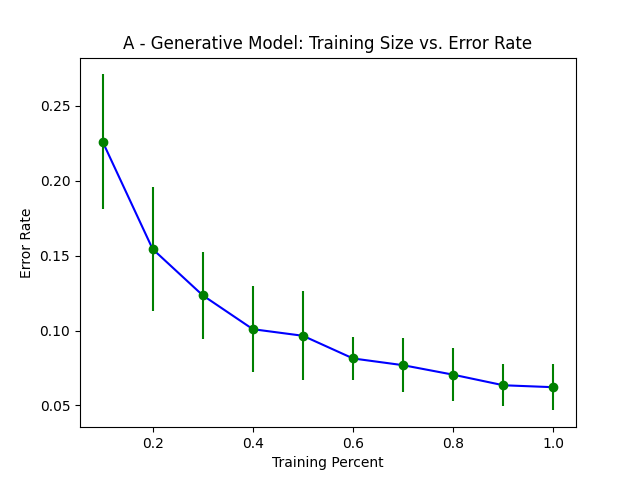
\includegraphics[width=0.5\textwidth]{../output/generative-A.png}
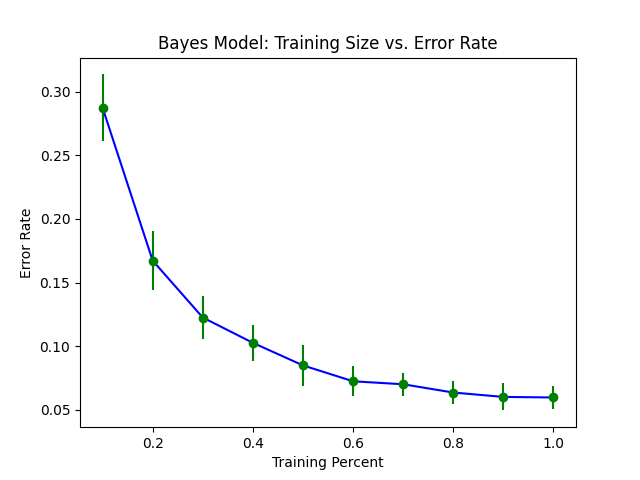
\includegraphics[width=0.5\textwidth]{../output/bayes-A.png}
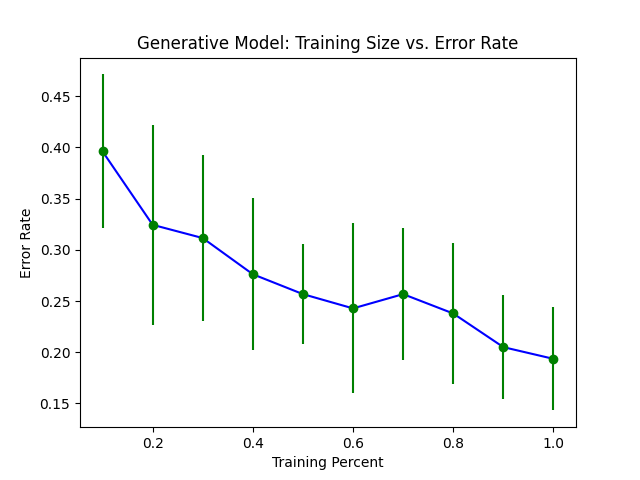
\includegraphics[width=0.5\textwidth]{../output/generative-B.png}
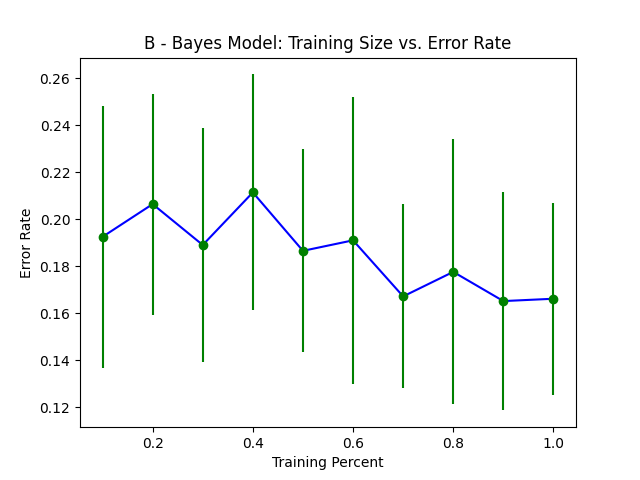
\includegraphics[width=0.5\textwidth]{../output/bayes-B.png}
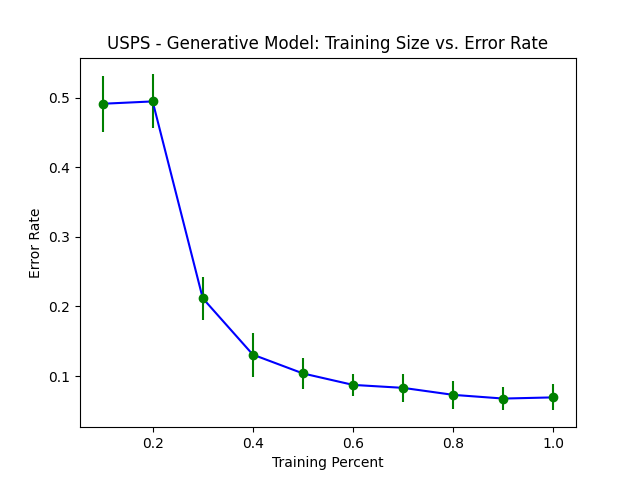
\includegraphics[width=0.5\textwidth]{../output/generative-USPS.png}
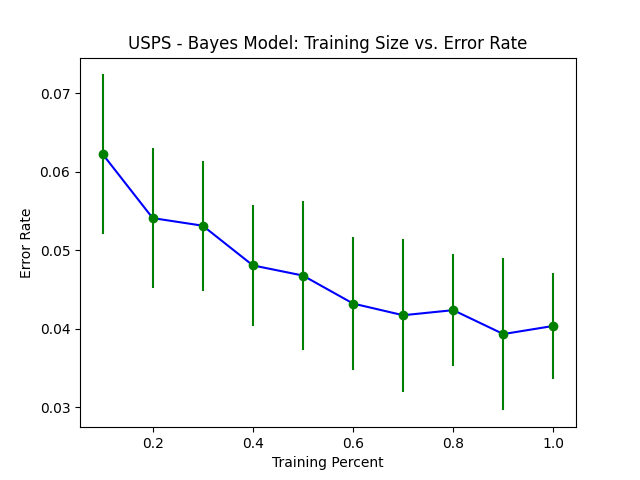
\includegraphics[width=0.5\textwidth]{../output/bayes-USPS.png}
\\ \\
Upon analyzing the data, it appears that the bayesian model's test error converges quicker and more steadily as a function of training size. This is likely due to the prior taken over the data which could help normalize the results under the random sampling.

\section*{Task 2)}

In the second task, we evaluate the convergence qualities of both newton's method and gradient ascent under the bayesian logistic regression model. This translates to analyzing the rate at which the weight vector converges in terms of time and the final weight vector itself. The results are given in the graph below.

\end{document}